\chapter{Experiments} \label{experiments}
We have carried out three experiments. The goal of the first two experiments was
to test some specific hyperparameter settings of our system. First, we compared
different sampling strategies (section \ref{sec:exp:sample}). Next, we
experimented with the usage of genetic operators (section \ref{sec:exp:genop}).
The last experiment encompasses runs of our system on the OpenML-CC18 benchmarking
suite.
% TODO cite

\section{Sampling strategies} \label{sec:exp:sample}
In section \ref{sec:scoresample} we presented two different sampling strategies
--- either a sample of the original dataset is generated for every individual
(\emph{per-ind}),
or only once per generation (\emph{per-gen}). The goal of this experiment was to test whether one
of the approaches is better.

The strategies were tested on three different datasets:
\begin{itemize}
\item wilt --- medium size dataset % TODO describe it
\item wine-quality-white --- medium size dataset % TODO describe
\item magic --- large dataset % TODO describe
\end{itemize}

Sample size was chosen proportionally to the dataset size. The evaluation method
was 10 times 10-fold cross-validation.

% TODO maybe one pyplot with 3 figures
% TODO check if it still is pdf/a :-) :-) :-)
\begin{figure}[ht]\centering
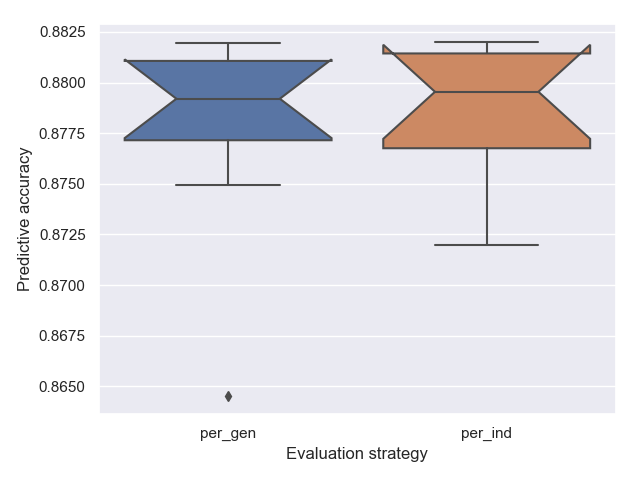
\includegraphics[width=0.7\textwidth]{../img/magic-out.png}
\caption{magic}
\label{pic04:magic}
\end{figure}

\begin{figure}[ht]\centering
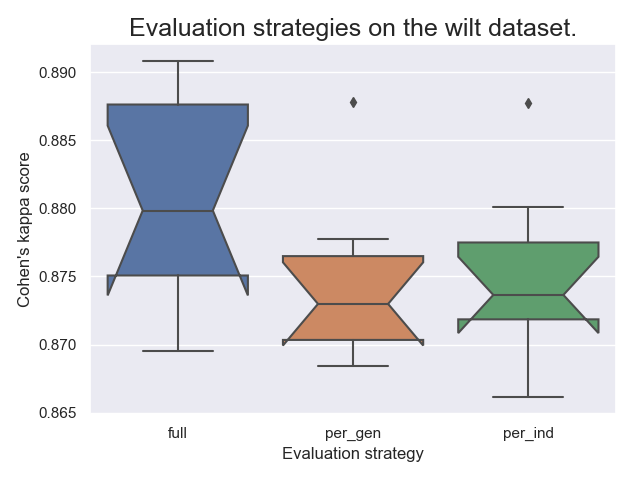
\includegraphics[width=0.7\textwidth]{../img/wilt-out.png}
\caption{wiltik}
\label{pic04:wilt}
\end{figure}

\begin{figure}[ht]\centering
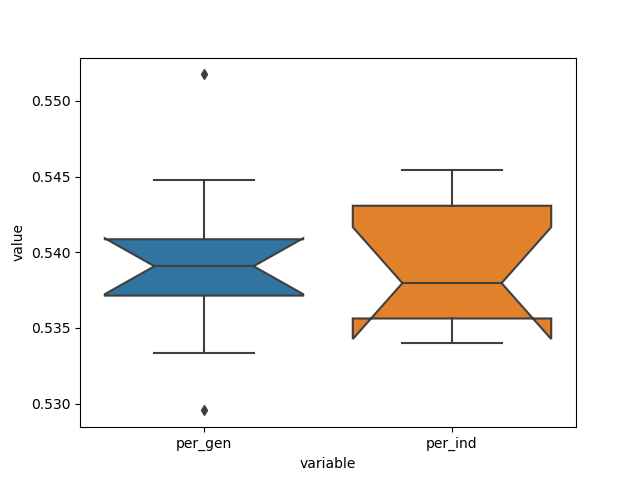
\includegraphics[width=0.7\textwidth]{../img/winequality-out.png}
\caption{wine-quality-white}
\label{pic04:winequality}
\end{figure}


% goal - test relationship between per gen and per ind

% Take maximum

% test comparison + describe

% boxplots for comparison (seaborn)
%   - winequality
%   - wilt
%   - magic

% scipt that gets the maximums and makes the plot(s)


\section{Combinations of genetic operators} \label{sec:exp:genop}


\section{OpenML-CC18 benchmarking suite}
% OpenML-CC18
% benchmark description